\documentclass[12pt, a4paper]{article}

\usepackage{polski}
\usepackage[utf8]{inputenc}
\usepackage[T1]{fontenc}
\usepackage{geometry}
\usepackage{graphicx}
\usepackage{fancyhdr}
\usepackage{amsmath}
\usepackage{amsfonts}
\usepackage{epstopdf}

\newgeometry{tmargin=2cm, bmargin=2cm, lmargin=2cm, rmargin=2cm}

\setlength{\parindent}{10mm}
\setlength{\parskip}{4mm}

\begin{document}
    
    \pagestyle{fancy}
    \renewcommand{\headrulewidth}{0pt}
    \renewcommand{\footrulewidth}{0.4pt}
    \fancyhead{}
    \lfoot{\textit{PKSS 2015/2016 --~Model budynku}}
    \cfoot{}
    \rfoot{\textit{Strona \thepage}}

	\setcounter{section}{0}
	\setcounter{page}{1}
    \section{Model budynku}
    \subsection{Opis modelu}
    \label{sec:opis_modelu}
    \indent
    
    Model budynku opierał się na dwóch równaniach różniczkowych, które opisują
    kaloryfery wewnątrz~\eqref{equ:radiator} (rozumiane jako jeden,
    ,,uśredniony'') oraz sam budynek wraz z~zawartym wewnątrz niego
    powietrzem~\eqref{equ:building} (wartości parametrów były identyczne jak
    w~dokumentacji):
	\begin{align}
		m_h c_h \frac{dT_{PCO}}{dt} & = F_{COB} \zeta c_w \left( T_{ZCO} - T_{PCO}
		\right) - k_h \left( T_{PCO} - T_r \right)
		\label{equ:radiator} \\
		m_b c_b \frac{dT_r}{dt} & = k_h \left( T_{PCO} - T_r \right) - k_{ext}
		\left( T_r - T_O \right)
		\label{equ:building}
	\end{align}
	
	Budynek posiadał swój własny regulator, którego zadaniem było utrzymanie
	stałej, ustalonej temperatury wewnątrz pomieszczeń. Wybrany został regulator PID
	w~postaci dyskretnej opisany równaniem:
	\begin{equation}
		u(t) = K_P \cdot e(t) + K_I \cdot h \cdot \sum\limits_{n=0}^{t} e(n) +
		K_D \cdot \frac{e(t) - e(t - 1)}{h}
		\label{equ:controller}
	\end{equation}
	gdzie $K_P$, $K_I$ oraz $K_D$ oznaczają wzmocnienia poszczególnych członów, zaś
	$h$ jest przyrostem czasu.
	
	Regulator sterował przeływem wody przez budynek, lecz przepływ ten nie mógł być
	nieograniczony i~mógł się zawierać w~przedziale od $0$ do
	$40$~[$\frac{m^3}{h}$]. Konieczne było zatem zastosowanie saturacji sygnału
	sterującego:
    \begin{equation}
		u_{sat}(t) =
		\begin{cases}
			0, & \mbox{gdy } u(t) \leq 0 \\
			u(t), & \mbox{gdy } u(t) \in (0; 1) \\
			1, & \mbox{gdy } u(t) \geq 1
		\end{cases}
		\label{equ:saturation}
    \end{equation}
    Wartość $u_{sat}$ rozumieć można jako poziom otwarcia zaworu sterującego
    przepływem wody, przez co równanie~\eqref{equ:radiator} zostało
    zmodyfikowane do postaci:
    \begin{equation}
		m_h c_h \frac{dT_{PCO}}{dt} = u_{sat} \cdot F_{COB} \zeta c_w \left( T_{ZCO}
		- T_{PCO} \right) - k_h \left( T_{PCO} - T_r \right)
		\label{equ:radiator_controller}
    \end{equation}
    
    \subsection{Opis implementacji}
    \label{sec:opis_implementacji}
    \indent
    
    Modele przedstawione w~poprzednim rozdziale zostały wykorzystane do
    napisania odpowiednich klas w~języku \textit{C++}. Do rozwiązywania równań
    różniczkowych wykorzystano metodę \textit{Runge-Kutta}.
    
    Komunikacja w~systemie wykorzystuje sockety TCP, dzięki czemu kod nie jest
    niepotrzebnie rozbudowany, a~jednocześnie umożliwia dwustronną komunikację
    sieciową. Transport danych został zrealizowany z~wykorzystaniem biblioteki
    \textit{rapidjson}, natomiast poszczególne pola składowe tych JSONów były
    zgodne z~ogólnie przyjętą dla całego projektu specyfikacją.
    
    \newpage
    
    \subsection{Platforma docelowa}
    \label{sec:platforma_docelowa}
    \indent
    
    Jako platforma docelowa wybrana została płytka \textit{Arduino Y\'un}, na
    pokładzie której dostępne są dwa mikrokontrolery. Pierwszy, z~rdzeniem
    \textit{megaAVR}, jest w~przypadku tego projektu niewykorzystywany. Drugi,
    z~rdzeniem \textit{MIPS}, jest wykorzystywany przez system \textit{OpenWRT}.
    System ten, oparty na jądrze \textit{Linux}, występuje powszechnie
    w~urządzeniach sieciowych takich jak routery, switche czy access pointy. Na
    tej płytce połączony jest z~gniazdem Ethernet oraz modułem WiFi.
    
    Dzięki dostępnymi w~systemie \textit{OpenWRT} podstawowymi narzędziami
    programistycznymi, takimi jak \textit{gcc} czy też \textit{make}, możliwe
    było tworzenie aplikacji docelowej na komputerze PC (w~trakcie testów), aby
    następnie móc przenieść ją na platformę docelową.
    
    Płytka \textit{Arduino Y\'un} stworzona została z~myślą o~internecie rzeczy
    (\textit{IoT}), dzięki czemu jednym z~możliwych scenariuszy rozwojowych tego
    projektu byłoby wykorzystanie tego układu do sterowania rzeczywistym
    procesem (a~także gromadzeniem danych na jego temat), zamiast modelowania
    go, a~następnie łączenie tych rozproszonych procesów w~zorganizowany system.
    
    \subsection{Dobór nastaw regulatora}
    \label{sec:dobor_nastaw}
    \indent
    
    W~celu doboru nastaw regulatora temperatury w~budynku, stworzony został,
    zgodnie z~równaniami przedstawionymi w~rozdziale~\ref{sec:opis_modelu},
    model budynku w~programie \textsc{Simulink}.
    
    \begin{figure}[!ht]
    	\centering
    	\includegraphics[width=10cm]{../img/model_simulink.png}
    	\caption{Model budynku stworzony w~programie \textsc{Simulink}}
    	\label{rys:model_simulink}
    \end{figure}
    
    Do doboru nastaw wykorzystano pierwszą metodę Zieglera-Nicholsa. W
    pierwszym kroku konieczne było otrzymanie odpowiedzi skokowej obiektu, która
    przedstawiona jest na rysunku~\ref{rys:odp_skokowa}. Odpowiedź ta uzyskana
    została przy założeniu stałej temperatury wody dopływającej do kaloryferów
    równej $70$~[$^oC$] oraz stałej temperatury otoczenia równej $0$~[$^oC$].
    Następnie wyznaczono punkt, w~którym pochodna odpowiedzi skokowej jest
    największa i~wyrysowano styczną do odpowiedzi w~tym punkcie. Kolejnym etapem
    było wyznaczenie parametrów obiektu --~stałej czasowej $T$ oraz opóźnienia
    $\tau$.
    
    \begin{figure}[!ht]
    	\centering
    	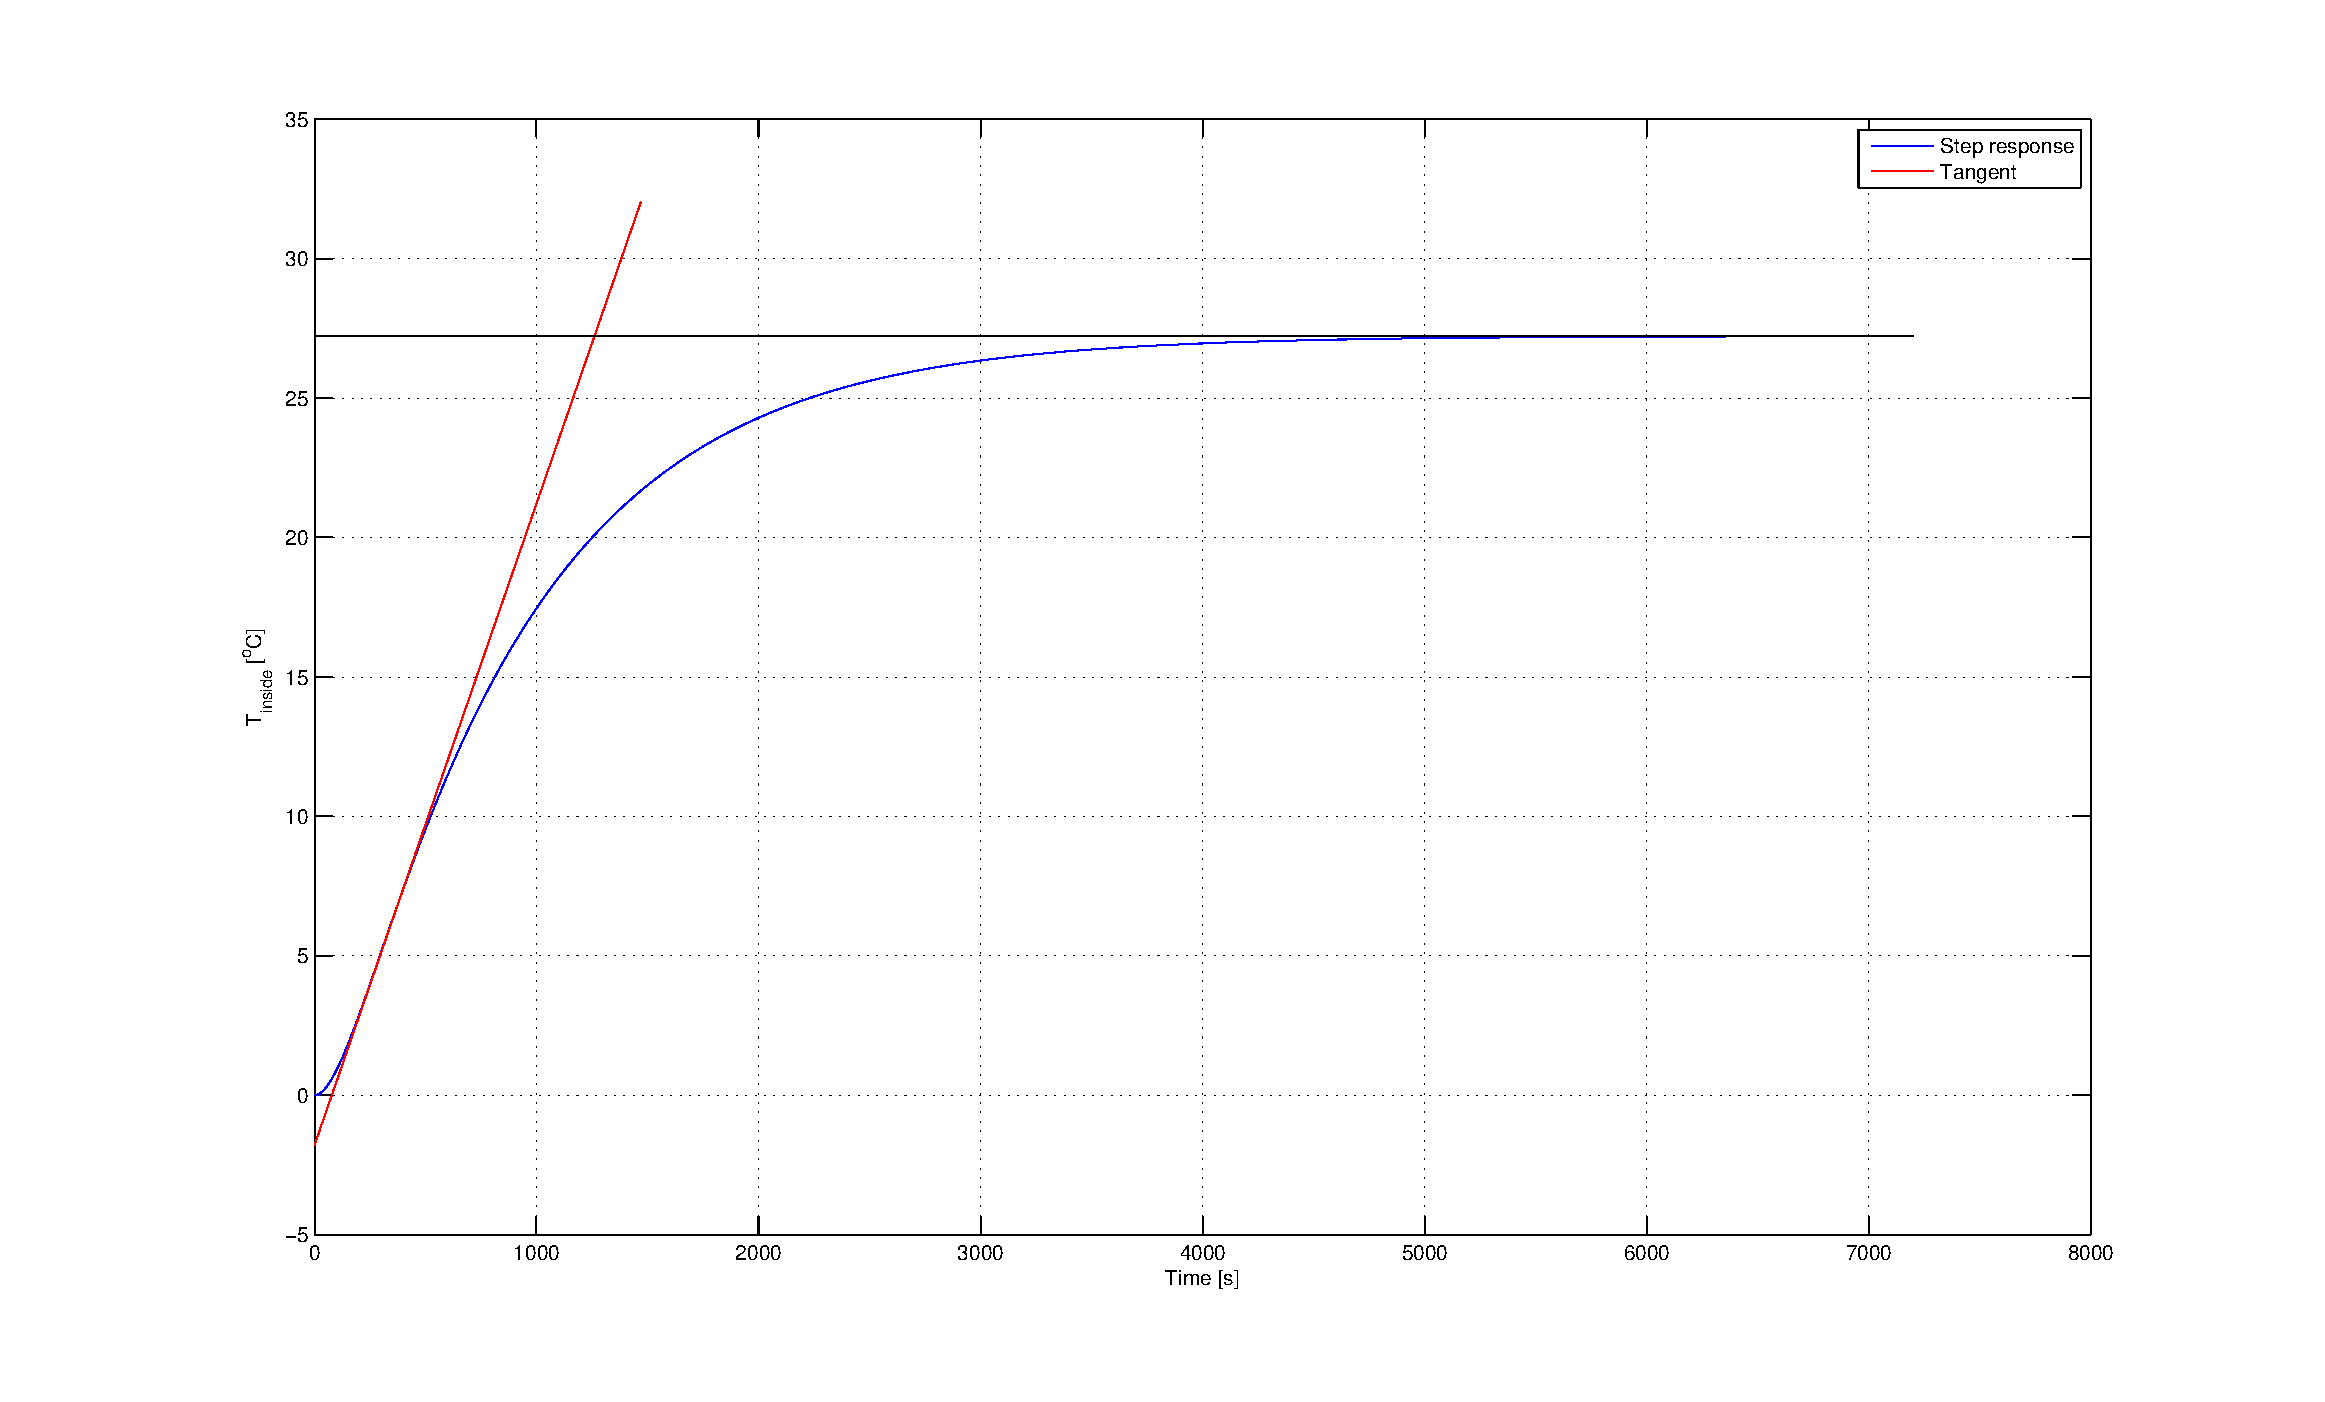
\includegraphics[width=\textwidth]{../img/odp_skokowa.eps}
    	\caption{Odpowiedź skokowa obiektu}
    	\label{rys:odp_skokowa}
    \end{figure}
    
    Na podstawie wyznaczonych parametrów, zgodnie z~tabelą dla pierwszej metody
    Z-N, dobrane zostały nastawy regulatora, które wynosiły:
    \begin{itemize}
        \item $K_P = 5.2$,
        \item $K_I = 0.028$,
        \item $K_D = 203$.
    \end{itemize}
    Podjęta została również próba doboru nastaw przy wykorzystaniu opcji
    \textit{Tune} w~programie \textsc{Matlab}. Nastawy otrzymane w~tym przypadku
    (po zaokrągleniu) wyniosły:
    \begin{itemize}
        \item $K_P = 0.5$,
        \item $K_I = 0.0005$,
        \item $K_D = 50$.
    \end{itemize}
    
    Przebiegi temperatury wewnątrz budynku dla obu zestawów przedstawione są na
    rysunku~\ref{rys:temp}. Widać wyraźnie, że pierwszy zestaw nastaw powoduje
    trwające długi czas oscylacje, co jest spowodowane ewidentnie zbyt duża
    wartością wzmocnienia części całkującej, która powoduje, w~połączeniu
    z~blokiem saturacji, że powstaje tzw. ,,windup''. Funkcja \textit{Tune}
    uwzględnia saturację (pracuje na modelu, który posiada ten blok), tak więc
    pozwala dobrać nastawy lepiej pasujące do konkretnego obiektu.
    
    \newpage
    
    \begin{figure}[!ht]
    	\centering
    	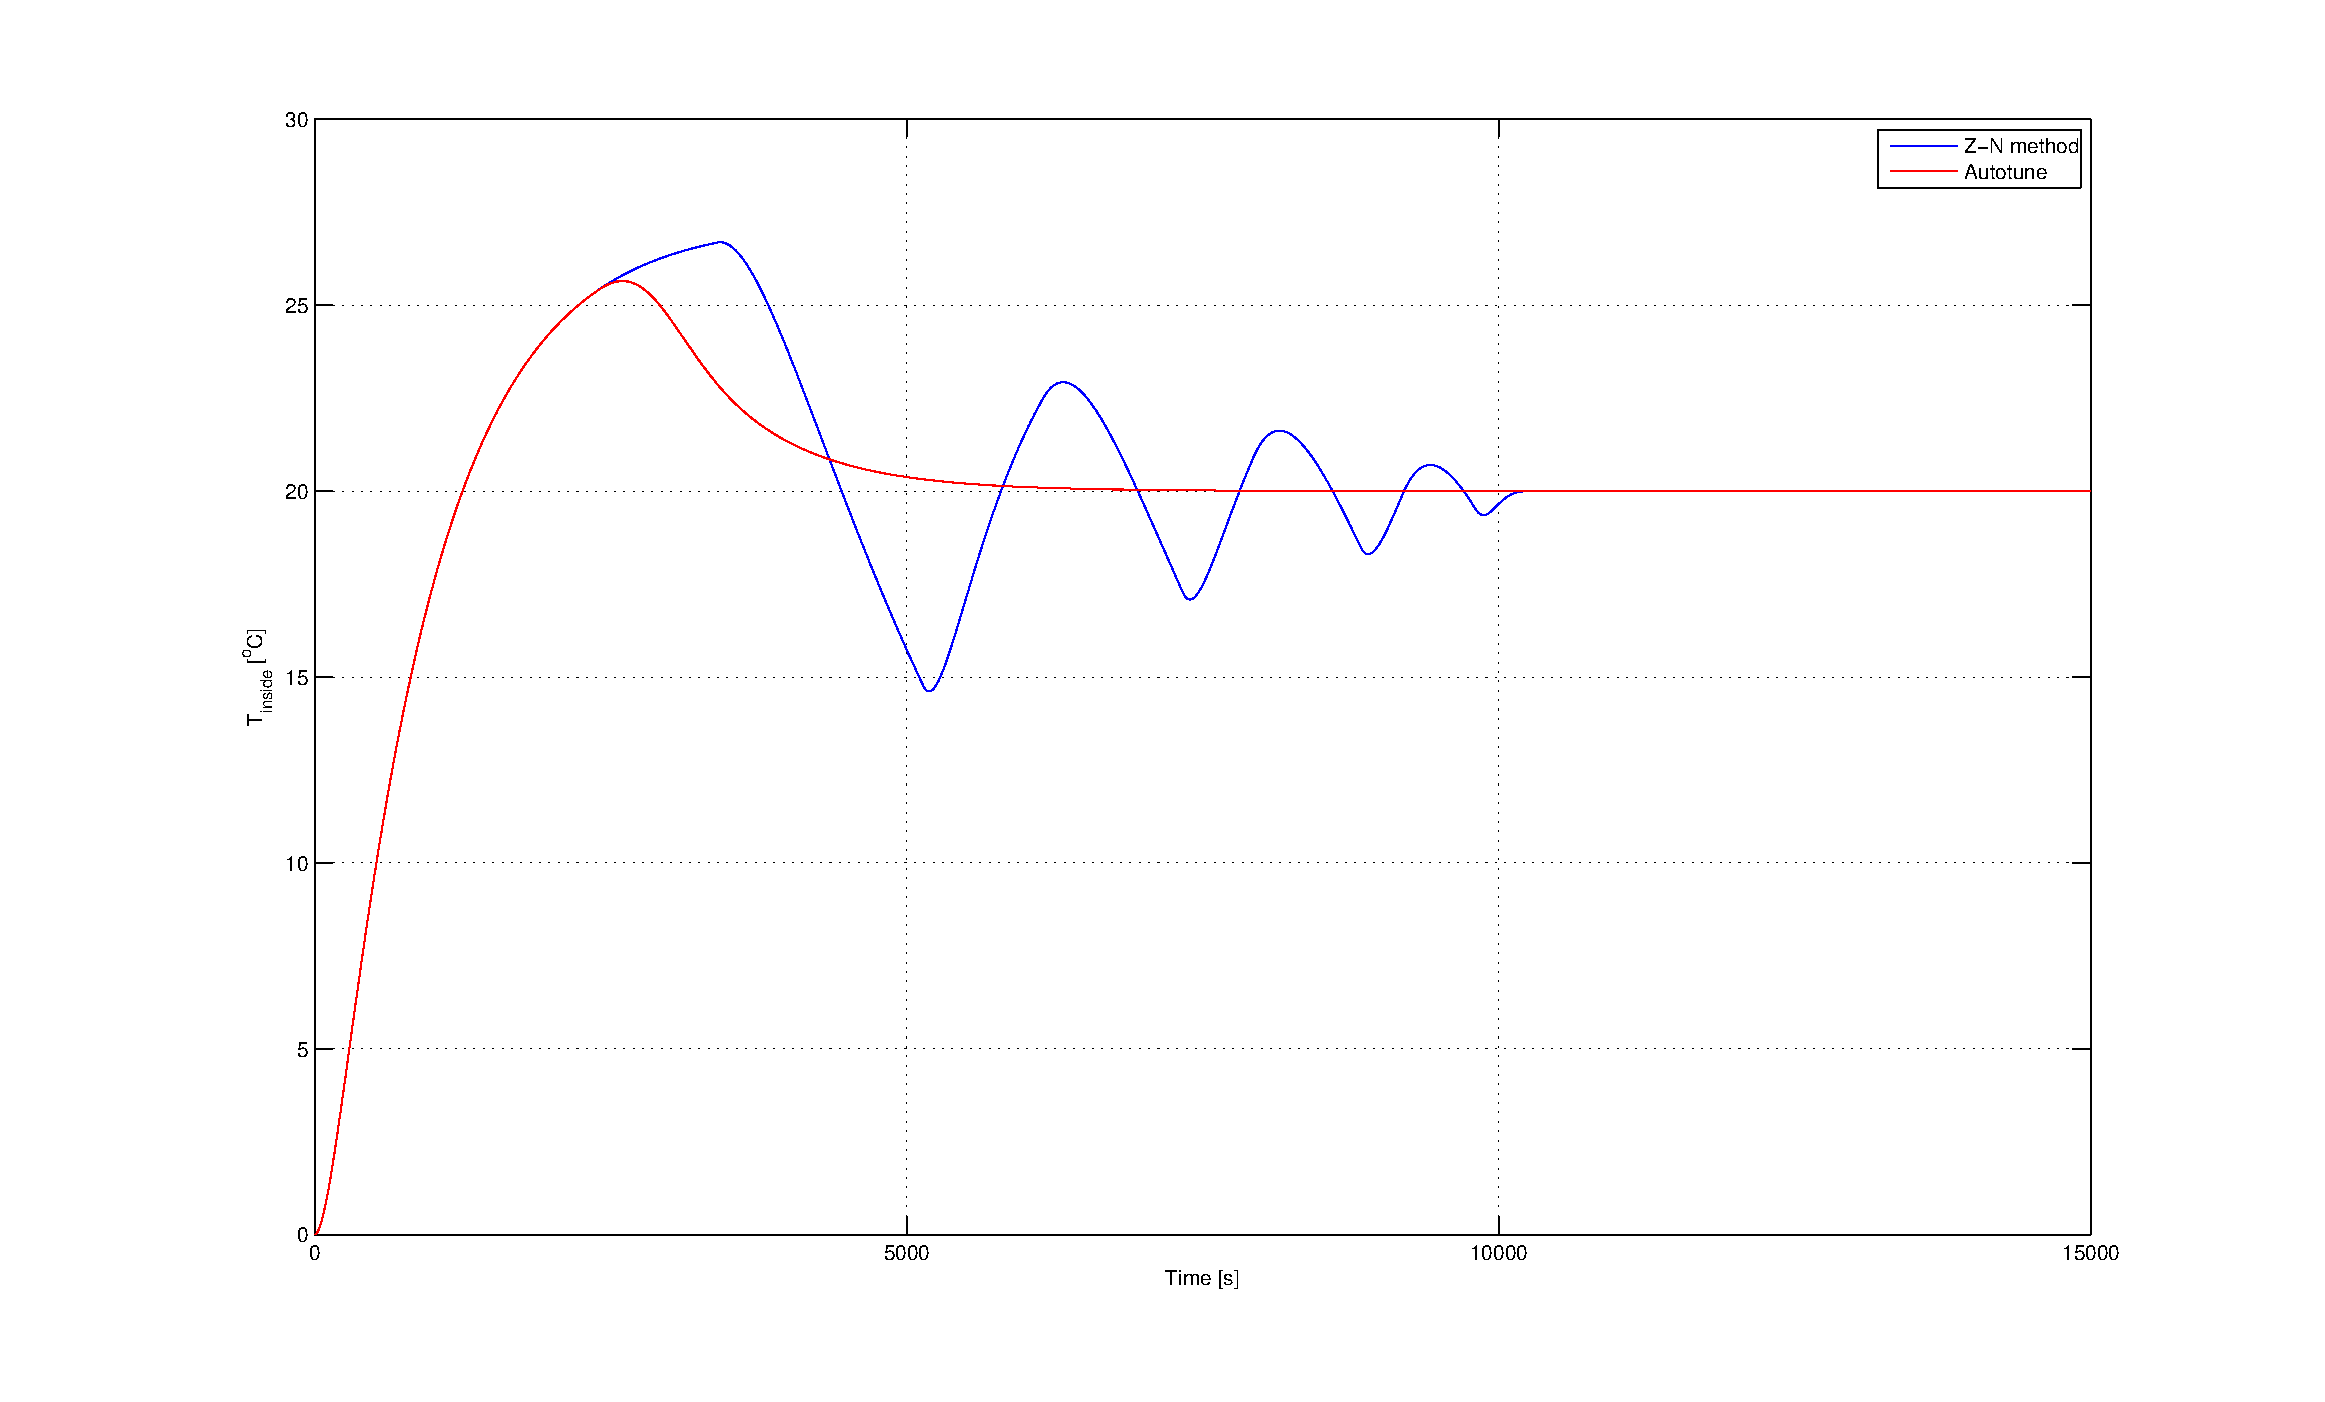
\includegraphics[width=\textwidth]{../img/temp.eps}
    	\caption{Przebiegi temperatury dla różnych nastaw regulatora}
    	\label{rys:temp}
    \end{figure}
    
    Przedstawione powyżej nastawy otrzymane zostały przy pewnych ograniczeniach
    związanych z~wartościami parametrów, które w~rzeczywistym systemie ulegają
    częstym zmianom, a~mianowicie wartość temperatury wody zasilającej oraz
    temperatury otoczenia. Mimo wszystko stanowią one dobry punkt wyjściowy do
    doboru nastaw regulatora w~całym systemie.
    
\end{document}
